% Beamer and More
\documentclass[12pt,hyperref=true,mathserif]{beamer}

% Package and Theme
\usepackage{amsmath}
\usetheme{AnnArbor}
\graphicspath{{Figure/}{figures/}{figure/}{pictures/}{picture/}{pic/}{pics/}}

% Document Begin
\begin{document}
\title[Miners to Millionaires]{From Miners to Millionaires}
\author{Yanan Xiao}
\institute[Masdar Institute]{Masdar Institute of Science and Technology}
\date[CIS501 Presentation]{Data Mining Course Presentation}

% Frame Begin
\begin{frame}
\titlepage~
\end{frame}

%\begin{frame}[shrink]
\begin{frame}
\tableofcontents
\end{frame}

\begin{frame}
\centering
``Theory and Practice were born together.''
\end{frame}

% Glossaries
\begin{frame}
\frametitle{Glossaries}
\begin{itemize}
  \item IR:\@ Information Retrieval\\[6pt]
  \item VSM:\@ Vector Space Model\\[6pt]
  \item JSM:\@ Jensen-Shannon Model\\[6pt]
  \item PCA:\@ Principal Component Analysis\\[6pt]
  \item Trustrace:\@ Trust-Based Traceability\\[6pt]
  \item TF/IDF:\@ Text Frequency and Inverse Document Frequency\\[6pt]
  \item MSW:\@ Multiple-Static Weights\\[8pt]
\end{itemize}
\end{frame}

\section{Introduction}
\begin{frame}
\frametitle{Definition of Traceability}
\begin{columns}
\begin{column}{0.5\textwidth}

\includegraphics[scale=0.75]{bounty-hunter-track}
\end{column}
\begin{column}{0.5\textwidth}
Traceability is the only means to ensure that the source code of a system is \textcolor{red}{consistent} with its requirements. \\
And that \textcolor{red}{all and only} the specified requirements have been implemented by developers.
\end{column}
\end{columns}
\end{frame}

\begin{frame}
\frametitle{Traceability Sad Facts}
\begin{columns}
\begin{column}{0.5\textwidth}
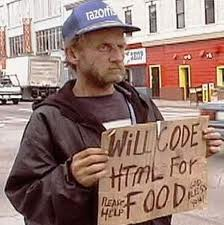
\includegraphics[scale=0.5]{code-for-food}
\end{column}
\begin{column}{0.5\textwidth}
During software maintenance and evolution, requirement traceability links become \textcolor{red}{obsolete}.\\
~\\
Because developers do not/cannot devote effort to updating them.
\end{column}
\end{columns}
\end{frame}

\begin{frame}
\begin{columns}
\begin{column}{0.5\textwidth}

\includegraphics[scale=0.25]{modern-miners}
\end{column}
\begin{column}{0.5\textwidth}
More sad: Recovering these traceability links later is a daunting and costly task for \textcolor{blue}{developers}.
\end{column}
\end{columns}
\end{frame}

\begin{frame}
\frametitle{State-of-the-Art Technique}
\begin{columns}
\begin{column}{0.5\textwidth}
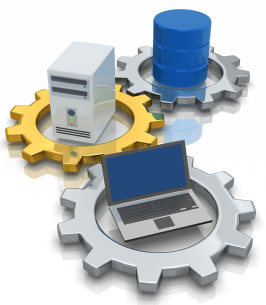
\includegraphics[scale=0.4]{Automation}
\end{column}
\begin{column}{0.5\textwidth}
The literature has proposed methods, techniques, and tools to recover these traceability links semi-automatically or automatically.\\
~\\
\textbf{Information Retrieval} (IR) techniques can \textcolor{red}{automatically} recover traceability links between free-text requirements and source code.
\end{column}
\end{columns}
\end{frame}

\section{Trustrace}
\begin{frame}
\frametitle{A Mathematician's Approach}
A set of requirements:
\begin{equation}
\label{equ:Requirements}
  R~=~\{r_{1},\ldots,r_{N}\}
\end{equation}
A set of classes:
\begin{equation}
\label{equ:Classes}
  C~=~\{c_{1},\ldots,c_{M}\}
\end{equation}
A collection of sets:
\begin{equation}
\label{equ:Sets}
  T~=~\{T_{1},\ldots,T_{P}\}
\end{equation}
where each $T_{i}~=~{T_{1},\ldots,T_{N_{i}}}$ is a set of homogeneous pieces of information.
\end{frame}

\begin{frame}
For each set $T_{i}\in T$, we build a set $R2CT_{i,r_{j},t_{k}}$ for each expert $T_{i}$ as follows:
\begin{equation}
\label{equ:RequirementSetforExperts}
  R2CT_{i,r_{j},t_{k}}~=~\{(r_{j},c_{s},\sigma^{'}_{i}(r_{j},t_{k}))|c_{s}\in \delta_{T_{i}}(t_{k}) \& t_{k}\in T_{i}\}
\end{equation}
And we use the sets $T_{i} \in T$ to build a set of trustable links $T_{r}$:

\begin{equation}
    \begin{array}{rcl}
        T_{r} & = & \{(r_{j},c_{s},\sigma^{'}_{i}(r_{j},t_{k}))|\\
                  &  & \exists t_{k} \in T_{i}:(r_{j},c_{s})\in \alpha(R2CT_{i,r_{j},t_{k}})\\
                  &  & \&(r_{j},c_{s}) \in \alpha(R2C)\}
    \end{array}
\end{equation}
In $TC_{i}(r_{j},c_{s})$ a new similarity $\sigma^{*}_{i}(r_{j},c_{s})$ computed as:
\begin{equation}
\label{equ:TrumoNewSimilarity}
  \sigma^{*}_{i}(r_{j},c_{s})~=~\frac{\sigma_{i}(r_{j},c_{s})+\sum_{l\in TC_{i}(r_{j},c_{s})}\phi(l)}{1+|TC_{i}(r_{j},c_{s})|}
\end{equation}
\end{frame}

\begin{frame}
Finally Trumo combine assigned value  to each link $T_{r}$ as follows:
\begin{equation}
    \begin{array}{rcl}
        \psi_{r_{j},c_{s}}(T_{r}) & = & [\sum_{i=1}^{P}\lambda_{i}(r_{j},c_{s})\sigma^{*}_{i}(r_{j},c_{s})]\\
        &  &  \\
                  &  & +\lambda_{P+1}(r_{j}c_{s}) \frac{|T_{r}(r_{j},c_{s})|}{max_{n,m}|T_{r}(r_{N},c_{M})|}\\

    \end{array}
\end{equation}
\end{frame}

\begin{frame}
\frametitle{An Architecture's Approach}
\begin{figure}
  \centering
  % Requires \usepackage{graphicx}
  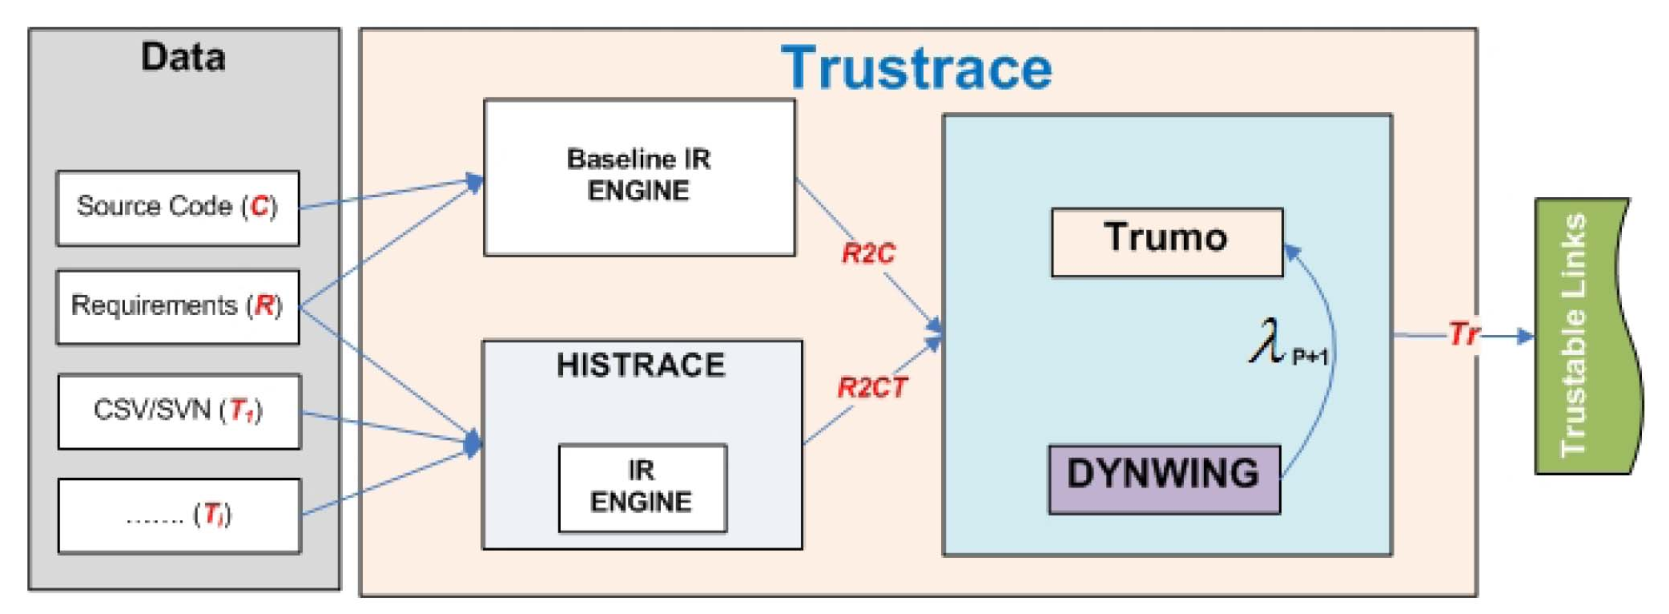
\includegraphics[scale=0.2]{Traceability}\\
  \caption{Trust-based requirement traceability process}\label{fig:Traceability}
\end{figure}
\end{frame}

\begin{frame}
\begin{figure}
  \centering
  % Requires \usepackage{graphicx}
  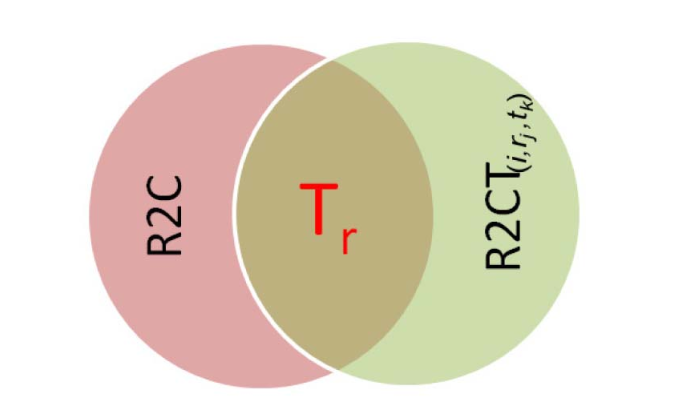
\includegraphics[scale=0.4]{Overlap}\\
  \caption{Overlapping of $R2C$, $R2CT_{i,r_{j},t_{k}}$ and $T_{r}$}\label{fig:Overlap}
\end{figure}
\end{frame}

\begin{frame}
\frametitle{Trustrace Step-by-Step}
\begin{itemize}
  \item \textcolor{red}{Histrace}: Uses requirements' textual descriptions, CVS/SVN commit messages, bug reports and classes to produce experts.\\[12pt]
  \item \textcolor{red}{Trumo}: Uses a web model of users' trust to discard and/or rerank the similarity of links in $T_{r}$.\\[12pt]
  \item \textcolor{red}{DynWing}: Uses Expectation-Maximization approach to choose the right weight per link for different experts.
\end{itemize}
\end{frame}

\subsection*{Technical Notes}


\begin{frame}[fragile,containsverbatim]
  \frametitle{Histrace}
  Histrace creates links between the set of requirements, $R$ and the
  source code, $C$, using the software repositories.\\
  In the following, $T_{1}$ stands for CVS/SVN commit messages, and
  $T_{2}$ for bug reports.\\[6pt]
  \begin{block}{Link each commit message and bug reports}
\begin{verbatim}
((b)[ug]{0,2}\s*[id]{0,3}|id|fix|pr|#)
[\s#=]*[?([0--9]{4,6})]?
\end{verbatim} 
  \end{block}
Tuned to the naming and numbering conventions by the developers of
\emph{Rhino}.
\end{frame}

\begin{frame}[fragile,containsverbatim]
  In the last step, Histrace removes false-positive links by imposing
  the following constraint:
  \begin{block}{Remove false-positive link with regular expression}
\begin{verbatim}
fix(e[ds])?|bugs?|problems?|defects?patch
\end{verbatim}
  \end{block}
\end{frame}

\begin{frame}
  \frametitle{IR Techniques}
  VSM and JSM are used by researchers. These techniques both
  essentially use term-by-document matrices. 
  \begin{itemize}
    \item Vector Space Model. The well-known TF/IDF measure is
      chosen. A document is a vector of TF/IDF weights. TF is the
      local weight whereas IDF a global weight of a term.
      \begin{equation}
        \label{eq:1}
        {(TF/IDF)}_{i,j}=\frac{n_{i,j}}{\sum_{k}n_{k,j}}*
        \log_{2}{(\frac{|D|}{|d:t_{i}\in d|})}
      \end{equation}
    \item Jensen-Shannon Model. JSM represents each document through a
      probability distribution, i.e., a normalized term-by-document
      matrix.
      \begin{equation}
        \label{eq:2}
        p=\frac{n(w,d)}{T_{d}}
      \end{equation}
      Just a fancy way of expressing \emph{word frequency}.
      
  \end{itemize}
\end{frame}


\begin{frame}
  JSM ranks target documents via the ``distance'' of their probability
  distribution to that of the source document.
\begin{equation}
        \label{eq:4}
        JSM(q,d)=H(\frac{p_{q}+p_{d}}{2})-\frac{H(p_{q}+H(p_{d}))}{2}
\end{equation}
\begin{equation}
  \label{eq:5}
  H(p)=\sum h(p(w))
\end{equation}
\begin{equation}
  \label{eq:6}
  h(x)=-x\log x
\end{equation}
$H(p)$ is the entropy of the probability distribution $p$, and $p_{q}$
and $p_{d}$ are the probability distribution of the two documents.
\end{frame}
\section{Empirical Evaluation}
\begin{frame}
\frametitle{Goal}
\begin{itemize}
  \item \textcolor{red}{Quality Focus}:  The accuracy of  Trustrace in terms of precision and recall. Also includes improvement by DynWing in terms of $F_{1}$ score.\\[8pt]
  \item \textcolor{red}{Perspective}: The perspective of practitioners interested in recovering traceability links with greater precision and recall values.
\end{itemize}
\end{frame}

\begin{frame}
\frametitle{Research Questions}
\textbf{Accuracy of traceability links}:
\begin{itemize}
  \item \textbf{RQ1} recovered by Trustrace compare with JSM and VSM.\\[8pt]
  \item \textbf{RQ2} recovered by DynWing compare with PCA.
\end{itemize}
\end{frame}

\begin{frame}
\frametitle{Analysis Method}
\begin{itemize}
  \item To answer \textbf{RQ1}, we perform several experiments with \textcolor{blue}{different threshold values} on the recovered links to perform statistical tests on the precision and recall values.\\[8pt]
  \item To answer \textbf{RQ2}, we use PCA and DynWing to \textcolor{blue}{assign weights} to the traceability links recovered using Trustrace.
\end{itemize}
\end{frame}


\section{Results}
\begin{frame}
\begin{itemize}
  \item \textbf{RQ1}: Trustrace helps to recover more correct links than IR techniques alone. \textcolor{red}{When two experts are available, Trustrace is always better.} In only one case and with just a single expert due to a lack of external source of information, did recall go down.\\[8pt]
  \item \textbf{RQ2}: DynWing \textcolor{red}{provides better weights for different experts than a PCA-based weighting technique.} However, it is possible that in some cases PCA-based weighting provides the same (but not better) results as DynWing.
\end{itemize}
\end{frame}

\begin{frame}
\begin{figure}
  \centering
  % Requires \usepackage{graphicx}
  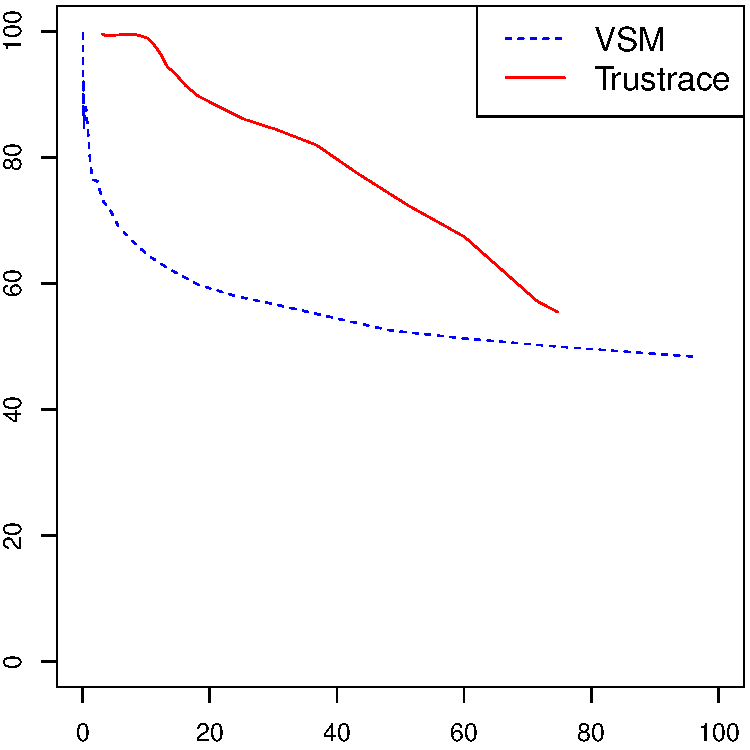
\includegraphics[scale=0.5]{js_normalised_rhino_2exp}\\
  \caption{Precision and recall values of JSM \& Trustrace, \textit{Rhino} example}\label{fig:JSMRhino}
\end{figure}
\end{frame}

\begin{frame}
\begin{figure}
  \centering
  % Requires \usepackage{graphicx}
  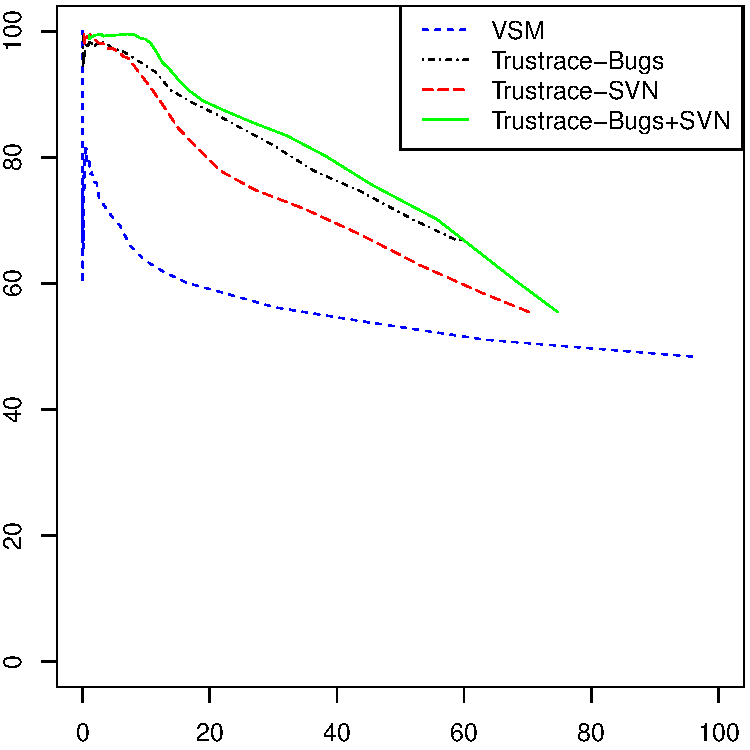
\includegraphics[scale=0.5]{vsm_rhino_2exp_example}\\
  \caption{Precision and recall values of VSM \& Trustrace, \textit{Rhino} example}\label{fig:VSMRhino}
\end{figure}
\end{frame}

\section{Discussion}
\begin{frame}
\begin{itemize}
  \item Data Set Quality Analysis\\[4pt]
  \item DynWing versus MSW versus PCA\\[4pt]
  \item Number of Experts\\[4pt]
  \item Other Observations\\[4pt]
  \item Practical Applicability Trustrace\\[4pt]
  \item Revisiting the Conjectures\\[4pt]
  \item Threats to Validity\\[4pt]
\end{itemize}
\end{frame}

\begin{frame}
\frametitle{Threats to Validity}
\begin{itemize}
  \item \textbf{Construct Validity}: Quantify the degree of inaccuracy by validation of the precision and recall using \textcolor{red}{manually built oracles}.\\[8pt]
  \item \textbf{Internal Validity}: Mitigate this threat by using \textcolor{red}{MSW- and PCA-generated $\lambda$ values}, and by using \textcolor{red}{the same setting} for all the experiments.\\[8pt]
  \item \textbf{External Validity}: The research approach is \textcolor{red}{applicable to any other systems}.\\[8pt]
  \item \textbf{Conclusion Validity}: Mitigate this threat by the appropriate nonparametric test \textcolor{red}{Mann-Whitney}. And applying \textcolor{red}{the Shapiro-Wilk} test to select data.
\end{itemize}
\end{frame}

\section{Future Work}
\begin{frame}
\begin{itemize}
  \item \textit{Histrace}: Implement more instances, using emails and forum discussions.\\[6pt]
  \item \textit{Trumo}: Use in other software engineering fields, in particular, test-case prioritization, anti-pattern detection and concept location.\\[6pt]
  \item \textit{Trustrace}: Deploy in a development environment. Perform experiments with real developers.\\[6pt]
  \item \textit{Regular Expression}: Use advanced matching techniques.\\[6pt]
\end{itemize}
\end{frame}

\begin{frame}
\begin{figure}
  \centering
  % Requires \usepackage{graphicx}
  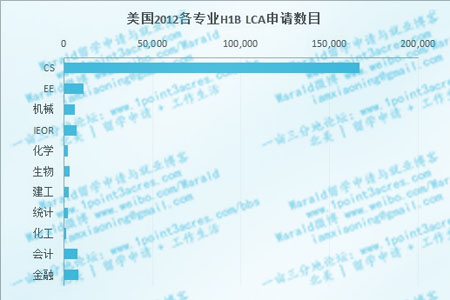
\includegraphics[scale=0.65]{H1B}\\
  \caption{Year 2012 H1B Applicants}\label{fig:H1B}
\end{figure}
\end{frame}

\begin{frame}
\begin{figure}
  \centering
  % Requires \usepackage{graphicx}
  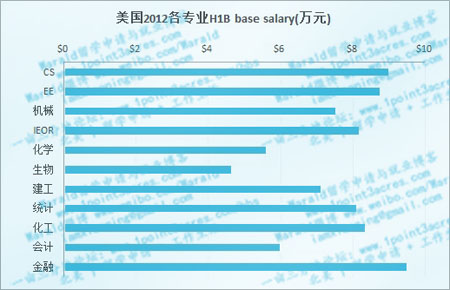
\includegraphics[scale=0.65]{Base-Salary}\\
  \caption{Year 2012 United States Base Salary, per Profession}\label{fig:BaseSalary}
\end{figure}
\end{frame}

\begin{frame}
\begin{figure}
  \centering
  % Requires \usepackage{graphicx}
  
\includegraphics[scale=0.45]{Question}\\
  \caption{No Question Off Limits!}\label{fig:QuestionandAnswer}
\end{figure}

\end{frame}
\end{document}



